\documentclass[a4paper]{article}
\usepackage{geometry}
\usepackage{graphicx}
\usepackage{natbib}
\usepackage{amsmath}
\usepackage{amssymb}
\usepackage{amsthm}
\usepackage{paralist}
\usepackage{epstopdf}
\usepackage{tabularx}
\usepackage{longtable}
\usepackage{multirow}
\usepackage{multicol}
\usepackage[hidelinks]{hyperref}
\usepackage{fancyvrb}
\usepackage{algorithm}
\usepackage{algorithmic}
\usepackage{float}
\usepackage{paralist}
\usepackage[svgname]{xcolor}
\usepackage{enumerate}
\usepackage{array}
\usepackage{times}
\usepackage{url}
\usepackage{fancyhdr}
\usepackage{comment}
\usepackage{environ}
\usepackage{times}
\usepackage{textcomp}
\usepackage{caption}
\usepackage{color}
\usepackage{xcolor}

\urlstyle{rm}

\setlength\parindent{0pt} % Removes all indentation from paragraphs
\theoremstyle{definition}
\newtheorem{definition}{Definition}[]
\newtheorem{conjecture}{Conjecture}[]
\newtheorem{example}{Example}[]
\newtheorem{theorem}{Theorem}[]
\newtheorem{lemma}{Lemma}
\newtheorem{proposition}{Proposition}
\newtheorem{corollary}{Corollary}

\floatname{algorithm}{Procedure}
\renewcommand{\algorithmicrequire}{\textbf{Input:}}
\renewcommand{\algorithmicensure}{\textbf{Output:}}
\newcommand{\abs}[1]{\lvert#1\rvert}
\newcommand{\norm}[1]{\lVert#1\rVert}
\newcommand{\RR}{\mathbb{R}}
\newcommand{\CC}{\mathbb{C}}
\newcommand{\Nat}{\mathbb{N}}
\newcommand{\br}[1]{\{#1\}}
\DeclareMathOperator*{\argmin}{arg\,min}
\DeclareMathOperator*{\argmax}{arg\,max}
\renewcommand{\qedsymbol}{$\blacksquare$}

\definecolor{dkgreen}{rgb}{0,0.6,0}
\definecolor{gray}{rgb}{0.5,0.5,0.5}
\definecolor{mauve}{rgb}{0.58,0,0.82}

\newcommand{\Var}{\mathrm{Var}}
\newcommand{\Cov}{\mathrm{Cov}}

\newcommand{\vc}[1]{\boldsymbol{#1}}
\newcommand{\xv}{\vc{x}}
\newcommand{\Sigmav}{\vc{\Sigma}}
\newcommand{\alphav}{\vc{\alpha}}
\newcommand{\muv}{\vc{\mu}}

\newcommand{\red}[1]{\textcolor{red}{#1}}

\def\x{\mathbf x}
\def\y{\mathbf y}
\def\w{\mathbf w}
\def\v{\mathbf v}
\def\E{\mathbb E}
\def\V{\mathbb V}

% TO SHOW SOLUTIONS, include following (else comment out):
\newenvironment{soln}{
    \leavevmode\color{blue}\ignorespaces
}{}


\hypersetup{
%    colorlinks,
    linkcolor={red!50!black},
    citecolor={blue!50!black},
    urlcolor={blue!80!black}
}

\geometry{
  top=1in,            % <-- you want to adjust this
  inner=1in,
  outer=1in,
  bottom=1in,
  headheight=3em,       % <-- and this
  headsep=2em,          % <-- and this
  footskip=3em,
}


\pagestyle{fancyplain}
\lhead{\fancyplain{}{Homework 2}}
\rhead{\fancyplain{}{CS 760 Machine Learning}}
\cfoot{\thepage}

\title{\textsc{Homework 2}} % Title

%%% NOTE:  Replace 'NAME HERE' etc., and delete any "\red{}" wrappers (so it won't show up as red)

\author{
\red{$>>$Jingxin Du$<<$} \\
\red{$>>$jdu86$<<$}\\
} 

\date{}

\begin{document}

\maketitle 


\textbf{Instructions:} 
Use this latex file as a template to develop your homework. Submit your homework on time as a single pdf file to Canvas. Please wrap your code and upload to a public GitHub repo, then attach the link below the instructions so that we can access it. You can choose any programming language (i.e. python, R, or MATLAB), as long as you implement the algorithm from scratch (e.g. do not use sklearn on questions 1 to 7 in section 2). Please check Piazza for updates about the homework.
{\color{blue}
\begin{verbatim}
    My public Github repo: https://github.com/pythonw-exe/CS760_HW2_DJX
\end{verbatim}
}
\section{A Simplified Decision Tree}
You are to implement a decision-tree learner for classification.
To simplify your work, this will not be a general purpose decision tree.  Instead, your program can assume that
\begin{itemize}
\item each item has two continuous features $\x \in \RR^2$
\item the class label is binary and encoded as $y \in \{0,1\}$
\item data files are in plaintext with one labeled item per line, separated by whitespace:
$$x_{11} \quad x_{12} \quad y_1$$
$$...$$
$$x_{n1} \quad x_{n2} \quad y_n$$
\end{itemize}

Your program should implement a decision tree learner according to the following guidelines:
\begin{itemize}
\item Candidate splits $(j,c)$ for numeric features should use a threshold $c$ in feature dimension $j$ in the form of $x_{\cdot j}\ge c$.
\item $c$ should be on values of that dimension present in the training data; i.e. the threshold is on training points, not in between training points. You may enumerate all features, and for each feature, use all possible values for that dimension.
\item You may skip those candidate splits with zero split information (i.e. the entropy of the split), and continue the enumeration.
\item The left branch of such a split is the ``then'' branch, and the right branch is ``else''.
\item Splits should be chosen using information gain ratio. If there is a tie you may break it arbitrarily.
\item The stopping criteria (for making a node into a leaf) are that 
	\begin{itemize}
	\item the node is empty, or
	\item all splits have zero gain ratio (if the entropy of the split is non-zero), or
	\item the entropy of any candidates split is zero
	\end{itemize}
\item To simplify, whenever there is no majority class in a leaf, let it predict $y=1$.
\end{itemize}

\section{Questions}
\begin{enumerate}
\item (Our algorithm stops at pure labels) [10 pts] If a node is not empty but contains training items with the same label, why is it guaranteed to become a leaf?  Explain. You may assume that the feature values of these items are not all the same. \\
{\color{blue}
Since a node contains training items with the same label, then the entropy of it is zero. Any further splits will result in zero entropy as well. (During this process, the information gain is also  zero). According to the algorithm's stopping criteria, criterion [3] - the entropy of any candidates split is zero is always satisfied. Therefore, it is guaranteed to become a leaf.
}

\item (Our algorithm is greedy)  [10 pts] Handcraft a small training set where both classes are present but the algorithm refuses to split; instead it makes the root a leaf and stop;
Importantly, if we were to manually force a split, the algorithm will happily continue splitting the data set further and produce a deeper tree with zero training error.
You should (1) plot your training set, (2) explain why.  Hint: you don't need more than a handful of items. \\
{\color{blue}
I selected four datapoints: (1,1,1), (1,5,0), (5,1,0), (5,5,1). Fig.\ref{Q2} shows my training set. For the root, the information gain ratio will be zero for any non-zero entropy spilt. According to the algorithm's stopping criterion [2]: all splits have zero gain ratio, so the root is now a leaf. However, if I manually force a split at (dimension = x2, cuts = 5), then for its sub tree, if I further split at (dimension = x1, cuts = 5), its  information gain ratio is non-zero, and the stopping criteria are not met, so the algorithm will happily continue splitting the data set further and produce a deeper tree. Eventually, all 4 points are divided into 4 different nodes in the tree, and thus the training error is zero.
}

\begin{figure}[htbp]
\centering
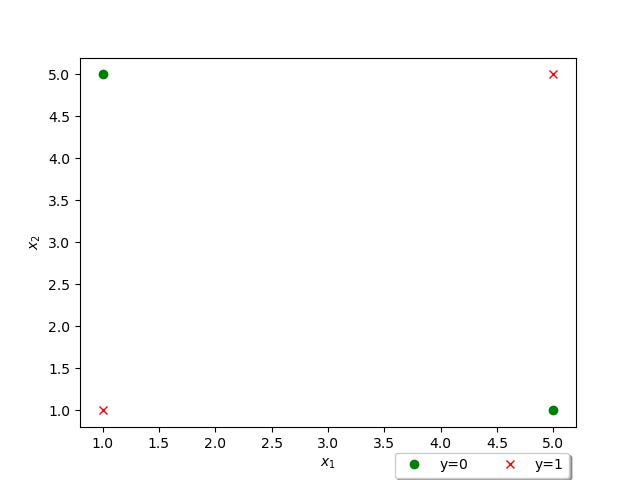
\includegraphics[width=4in]{Q2.jpg}
\caption{Training set plot}
\label{Q2}
\end{figure}

\item (Information gain ratio exercise)  [10 pts] Use the training set Druns.txt.  For the root node, list all candidate cuts and their information gain ratio. If the entropy of the candidate split is zero, please list its mutual information (i.e. information gain). Hint: to get $\log_2(x)$ when your programming language may be using a different base, use \verb|log(x)/log(2)|. Also, please follow the split rule in the first section. \\
{\color{blue}
I have attached all candidate cuts and their info gain ratio for the root node below:
\begin{verbatim}
[cal_info_gain_ratio] info gain ratio zero, info gain instead 0.0
[find_best_split] feature x1   threshold 0.0   info_gain_ratio 0
[find_best_split] feature x1   threshold 0.1   info_gain_ratio 0.10051807676021828
[cal_info_gain_ratio] info gain ratio zero, info gain instead 0.0
[find_best_split] feature x2   threshold -2.0   info_gain_ratio 0
[find_best_split] feature x2   threshold -1.0   info_gain_ratio 0.10051807676021828
[find_best_split] feature x2   threshold 0.0   info_gain_ratio 0.055953759631263526
[find_best_split] feature x2   threshold 1.0   info_gain_ratio 0.00578004220515232
[find_best_split] feature x2   threshold 2.0   info_gain_ratio 0.0011443495172767494
[find_best_split] feature x2   threshold 3.0   info_gain_ratio 0.016411136842102134
[find_best_split] feature x2   threshold 4.0   info_gain_ratio 0.049749064181778546
[find_best_split] feature x2   threshold 5.0   info_gain_ratio 0.11124029586339801
[find_best_split] feature x2   threshold 6.0   info_gain_ratio 0.23609960614360798
[find_best_split] feature x2   threshold 7.0   info_gain_ratio 0.055953759631263526
[find_best_split] feature x2   threshold 8.0   info_gain_ratio 0.4301569161309807
\end{verbatim}
}
\item (The king of interpretability)  [10 pts] Decision tree is not the most accurate classifier in general.  However, it persists.  This is largely due to its rumored interpretability: a data scientist can easily explain a tree to a non-data scientist.  Build a tree from D3leaves.txt.  Then manually convert your tree to a set of logic rules.  Show the tree\footnote{When we say show the tree, we mean either the standard computer science tree view, or some crude plaintext representation of the tree -- as long as you explain the format.  When we say visualize the tree, we mean a plot in the 2D $\x$ space that shows how the tree will classify any points.} and the rules. \\

{\color{blue}
The tree of Q4 is shown below:
\begin{verbatim}
     -node- feature: x2 cut: 2.0
     -left_subtree-
         -node- feature: x1 cut: 10.0
         -left_subtree-
             -leaf- prediction: 0
         -right_subtree-
             -leaf- prediction: 1
     -right_subtree-
         -leaf- prediction: 1
\end{verbatim}
The logical rules are shown below:

For my tree format, more indentation means deeper nodes, nodes/leaves that are at the same level in a tree have the same indentation. Left and right sub-tree of a node (relationships between nodes) are stated. Splitting dimension and threshold (internal node) and prediction (leaf) also are explicitly stated.

\begin{verbatim}
if x2 >= 2 then
    predicts y = 1
else
    if x1 >= 10 then predicts y = 1
    else predicts y = 0
\end{verbatim}
}

\item (Or is it?)  [20 pts] For this question only, make sure you DO NOT VISUALIZE the data sets or plot your tree's decision boundary in the 2D $\x$ space.  If your code does that, turn it off before proceeding.  This is because you want to see your own reaction when trying to interpret a tree.  You will get points no matter what your interpretation is.
And we will ask you to visualize them in the next question anyway.
  \begin{itemize}
  
  \item Build a decision tree on D1.txt.  Show it to us in any format (e.g. could be a standard binary tree with nodes and arrows, and denote the rule at each leaf node; or as simple as plaintext output where each line represents a node with appropriate line number pointers to child nodes; whatever is convenient for you). Again, do not visualize the data set or the tree in the $\x$ input space.  In real tasks you will not be able to visualize the whole high dimensional input space anyway, so we don't want you to ``cheat'' here. 

  {\color{blue}
The D1 decision tree is shown below:
\begin{verbatim}
     -node- feature: x2 cut: 0.201829
     -left_subtree-
         -leaf- prediction: 0
     -right_subtree-
         -leaf- prediction: 1
\end{verbatim}
}
  \item Look at your tree in the above format (remember, you should not visualize the 2D dataset or your tree's decision boundary) and try to interpret the decision boundary in human understandable English. 

{\color{blue}
Similar to Q4, I interpret the decision boundary in human understandable English using logical rules:
\begin{verbatim}
if x2 >= 0.201829 then
    predicts y = 1
else
    predicts y = 0
\end{verbatim}
}
  \item Build a decision tree on D2.txt.  Show it to us.
  
{\color{blue}
The D2 decision tree is shown below:
\begin{verbatim}
     -node- feature: x1 cut: 0.533076
     -left_subtree-
         -node- feature: x2 cut: 0.88635
         -left_subtree-
             -node- feature: x2 cut: 0.691474
             -left_subtree-
                 -node- feature: x2 cut: 0.534979
                 -left_subtree-
                     -leaf- prediction: 0
                 -right_subtree-
                     -node- feature: x1 cut: 0.426073
                     -left_subtree-
                         -node- feature: x1 cut: 0.409972
                         -left_subtree-
                             -node- feature: x1 cut: 0.393227
                             -left_subtree-
                                 -leaf- prediction: 0
                             -right_subtree-
                                 -node- feature: x2 cut: 0.639018
                                 -left_subtree-
                                     -leaf- prediction: 0
                                 -right_subtree-
                                     -leaf- prediction: 1
                         -right_subtree-
                             -node- feature: x2 cut: 0.597713
                             -left_subtree-
                                 -leaf- prediction: 0
                             -right_subtree-
                                 -leaf- prediction: 1
                     -right_subtree-
                         -leaf- prediction: 1
             -right_subtree-
                 -node- feature: x1 cut: 0.254049
                 -left_subtree-
                     -node- feature: x1 cut: 0.191915
                     -left_subtree-
                         -node- feature: x2 cut: 0.864128
                         -left_subtree-
                             -leaf- prediction: 0
                         -right_subtree-
                             -node- feature: x2 cut: 0.865999
                             -left_subtree-
                                 -leaf- prediction: 1
                             -right_subtree-
                                 -leaf- prediction: 0
                     -right_subtree-
                         -node- feature: x2 cut: 0.792752
                         -left_subtree-
                             -leaf- prediction: 0
                         -right_subtree-
                             -leaf- prediction: 1
                 -right_subtree-
                     -leaf- prediction: 1
         -right_subtree-
             -node- feature: x1 cut: 0.041245
             -left_subtree-
                 -leaf- prediction: 0
             -right_subtree-
                 -node- feature: x1 cut: 0.104043
                 -left_subtree-
                     -node- feature: x2 cut: 0.964767
                     -left_subtree-
                         -leaf- prediction: 0
                     -right_subtree-
                         -leaf- prediction: 1
                 -right_subtree-
                     -leaf- prediction: 1
     -right_subtree-
         -node- feature: x2 cut: 0.228007
         -left_subtree-
             -node- feature: x1 cut: 0.887224
             -left_subtree-
                 -node- feature: x1 cut: 0.850316
                 -left_subtree-
                     -leaf- prediction: 0
                 -right_subtree-
                     -node- feature: x2 cut: 0.169053
                     -left_subtree-
                         -leaf- prediction: 0
                     -right_subtree-
                         -leaf- prediction: 1
             -right_subtree-
                 -node- feature: x2 cut: 0.037708
                 -left_subtree-
                     -leaf- prediction: 0
                 -right_subtree-
                     -node- feature: x2 cut: 0.082895
                     -left_subtree-
                         -node- feature: x1 cut: 0.960783
                         -left_subtree-
                             -leaf- prediction: 0
                         -right_subtree-
                             -leaf- prediction: 1
                     -right_subtree-
                         -leaf- prediction: 1
         -right_subtree-
             -node- feature: x2 cut: 0.424906
             -left_subtree-
                 -node- feature: x1 cut: 0.708127
                 -left_subtree-
                     -node- feature: x2 cut: 0.32625
                     -left_subtree-
                         -leaf- prediction: 0
                     -right_subtree-
                         -node- feature: x1 cut: 0.595471
                         -left_subtree-
                             -leaf- prediction: 0
                         -right_subtree-
                             -node- feature: x1 cut: 0.646007
                             -left_subtree-
                                 -node- feature: x2 cut: 0.403494
                                 -left_subtree-
                                     -leaf- prediction: 0
                                 -right_subtree-
                                     -leaf- prediction: 1
                             -right_subtree-
                                 -leaf- prediction: 1
                 -right_subtree-
                     -leaf- prediction: 1
             -right_subtree-
                 -leaf- prediction: 1
\end{verbatim}
}

  \item Try to interpret your D2 decision tree. Is it easy or possible to do so without visualization? \\
  {\color{blue} The interpretation technique for D2 decision tree should be pretty similar to the previous D1 decision tree. However, D2 decision tree is very complicated, thus it is very hard for human beings to interpret it without visualization. Visualization can better demonstrate the results.}
  \end{itemize}

\item (Hypothesis space)  [10 pts] For D1.txt and D2.txt, do the following separately:
  \begin{itemize}
  
  \item Produce a scatter plot of the data set.

{\color{blue}
The scatter plots of data set D1 and D2 are shown in Fig.\ref{Q6-1} and Fig.\ref{Q6-2} respectively.
}

\begin{figure}[htbp]
\centering
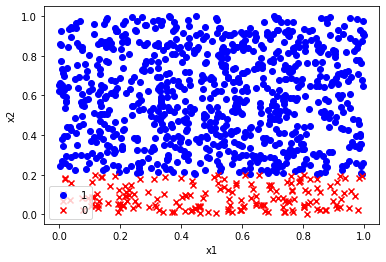
\includegraphics[width=4in]{Q6-1.png}
\caption{Scatter plot of D1}
\label{Q6-1}
\end{figure}

\begin{figure}[htbp]
\centering
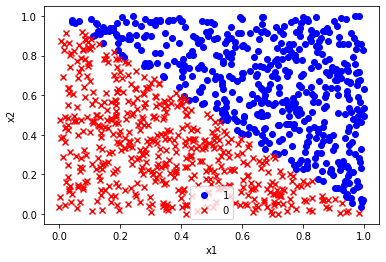
\includegraphics[width=4in]{Q6-2.png}
\caption{Scatter plot of D2}
\label{Q6-2}
\end{figure}

  \item Visualize your decision tree's decision boundary (or decision region, or some other ways to clearly visualize how your decision tree will make decisions in the feature space).

{\color{blue}
The decision boundary visualization of data set D1 and D2 are shown in Fig.\ref{Q6-3} and Fig.\ref{Q6-4} respectively.
}

\begin{figure}[htbp]
\centering
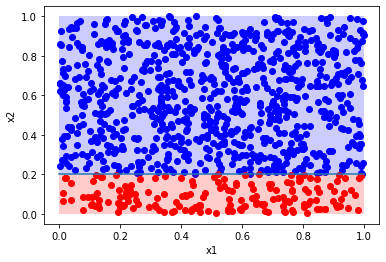
\includegraphics[width=4in]{Q6-3.png}
\caption{Decision boundary of D1}
\label{Q6-3}
\end{figure}

\begin{figure}[htbp]
\centering
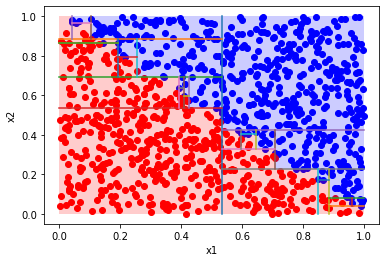
\includegraphics[width=4in]{Q6-4.png}
\caption{Decision boundary of D2}
\label{Q6-4}
\end{figure}

  \end{itemize}
Then discuss why the size of your decision trees on D1 and D2 differ.  Relate this to the hypothesis space of our decision tree algorithm. \\
{\color{blue}
For D1, we can find a clear decision boundary which is parallel to the x axis that can differentiate the data-set. However, for D2, even through its boundary is also obvious, there are no direct vertical or horizontal lines that can differentiate the data-set. As a result, the decision tree can easily be built for D1, but needs a lot of cuts parallel to the axis to predict data in D2, which makes D2 decision tree much more complicated.}

\item (Learning curve)  [20 pts] We provide a data set Dbig.txt with 10000 labeled items.  Caution: Dbig.txt is sorted.
  \begin{itemize}
  
  \item You will randomly split Dbig.txt into a candidate training set of 8192 items and a test set (the rest).  Do this by generating a random permutation, and split at 8192.
  
  \item Generate a sequence of five nested training sets $D_{32} \subset D_{128} \subset D_{512} \subset D_{2048} \subset D_{8192}$ from the candidate training set.  The subscript $n$ in $D_n$ denotes training set size.  The easiest way is to take the first $n$ items from the (same) permutation above.  This sequence simulates the real world situation where you obtain more and more training data.
  
  \item For each $D_n$ above, train a decision tree.  Measure its test set error $err_n$.  Show three things in your answer: (1) List $n$, number of nodes in that tree, $err_n$. (2) Plot $n$ vs. $err_n$.  This is known as a learning curve (a single plot). (3) Visualize your decision trees' decision boundary (five plots). \\
  \end{itemize}
  
\end{enumerate}

{\color{blue}

(1) I have listed $n$, number of nodes in that tree, and $err_{n}$ below:

\begin{verbatim}
D32, n=32:
    number of nodes: 3, error: 0.236
D128, n=128:
    number of nodes: 16, error: 0.073
D512, n=512:
    number of nodes: 31, error: 0.050
D2048, n=2048:
    number of nodes: 70, error: 0.030
D8192, n=8192:
    number of nodes: 126, error: 0.014
\end{verbatim}

(2) The learning curve ($n$ vs $err_{n}$) is shown below in Fig. \ref{Q7-6}.

(3) The visualizations of my decision trees' decision boundary are shown below in Fig. \ref{Q7-1}, Fig. \ref{Q7-2}, Fig. \ref{Q7-3}, Fig. \ref{Q7-4}, and Fig. \ref{Q7-5}.
}

\begin{figure}[htbp]
\centering
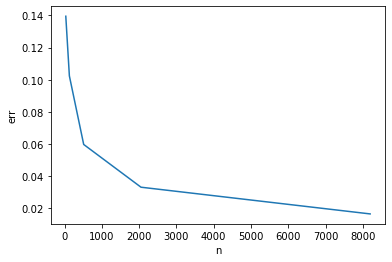
\includegraphics[width=4in]{Q7-6.png}
\caption{$n$ vs $err_{n}$}
\label{Q7-6}
\end{figure}

\begin{figure}[htbp]
\centering
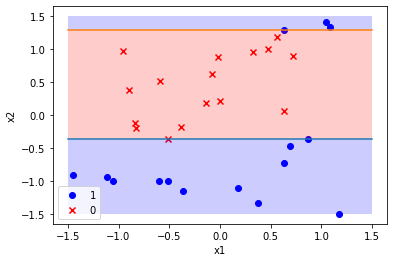
\includegraphics[width=4in]{Q7-1.png}
\caption{Decision boundary of $D_{32}$}
\label{Q7-1}
\end{figure}

\begin{figure}[htbp]
\centering
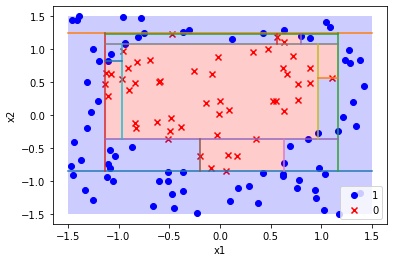
\includegraphics[width=4in]{Q7-2.png}
\caption{Decision boundary of $D_{128}$}
\label{Q7-2}
\end{figure}

\begin{figure}[htbp]
\centering
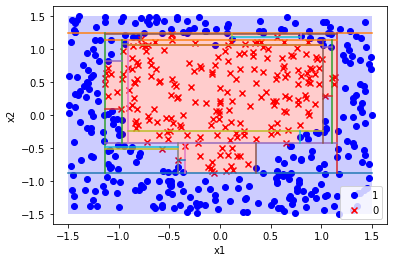
\includegraphics[width=4in]{Q7-3.png}
\caption{Decision boundary of $D_{512}$}
\label{Q7-3}
\end{figure}

\begin{figure}[htbp]
\centering
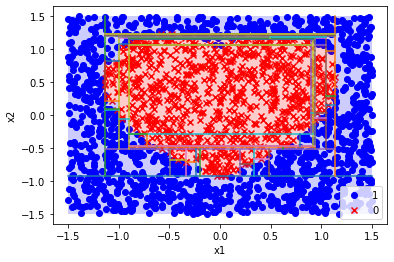
\includegraphics[width=4in]{Q7-4.png}
\caption{Decision boundary of $D_{2048}$}
\label{Q7-4}
\end{figure}

\begin{figure}[htbp]
\centering
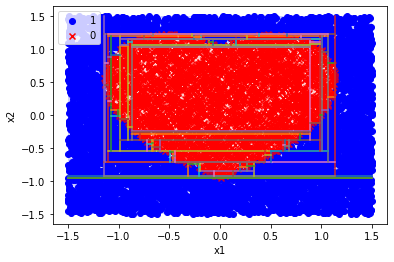
\includegraphics[width=4in]{Q7-5.png}
\caption{Decision boundary of $D_{8192}$}
\label{Q7-5}
\end{figure}

\section{sklearn [10 pts]}
Learn to use sklearn (\url{https://scikit-learn.org/stable/}).
Use sklearn.tree.DecisionTreeClassifier to produce trees for datasets $D_{32}, D_{128}, D_{512}, D_{2048}, D_{8192}$.  Show two things in your answer: (1) List $n$, number of nodes in that tree, $err_n$. (2) Plot $n$ vs. $err_n$.

{\color{blue}

(1) I have listed $n$, number of nodes in that tree, and $err_{n}$ below:

\begin{verbatim}
D32, n=32:
    number of nodes: 7, error: 0.139
D128, n=128:
    number of nodes: 14, error: 0.102
D512, n=512:
    number of nodes: 31, error: 0.060
D2048, n=2048:
    number of nodes: 68, error: 0.033
D8192, n=8192:
    number of nodes: 148, error: 0.017
\end{verbatim}

(2) The learning curve ($n$ vs $err_{n}$) is shown below in Fig. \ref{P3}.
}

\begin{figure}[htbp]
\centering
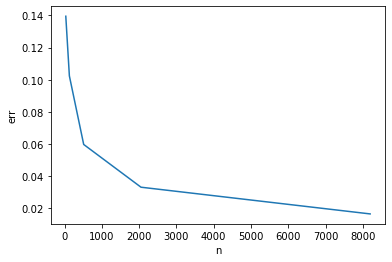
\includegraphics[width=4in]{P3.png}
\caption{$n$ vs $err_{n}$}
\label{P3}
\end{figure}

\section{Lagrange Interpolation [10 pts]}
Fix some interval $[a, b]$ and sample $n = 100$ points $x$ from this interval uniformly. Use these to build a training set consisting of $n$ pairs $(x, y)$ by setting function $y = sin(x)$. \\

Build a model $f$ by using Lagrange interpolation, check more details in \url{https://en.wikipedia.org/wiki/Lagrange_polynomial} and \url{https://docs.scipy.org/doc/scipy/reference/generated/scipy.interpolate.lagrange.html}. \\

Generate a test set using the same distribution as your test set. Compute and report the resulting model’s train and test error. What do you observe?
Repeat the experiment with zero-mean Gaussian noise $\epsilon$ added to $x$. Vary the standard deviation for $\epsilon$ and report your findings.

{\color{blue}
\begin{verbatim}
Initial
Train error: 0.004679452011714328
Test error: 0.004679452011714328
Epsilon: 0.5
Train error: 0.00046540904490213834
Test error: 0.00023323089445525223
Epsilon: 1.0
Train error: 13567.793928245372
Test error: 38694.61614936578
Epsilon: 4.0
Train error: 1.2037417284240464
Test error: 30.57729456236557
\end{verbatim}

I have attached a set of model's training and testing error I calculated. I notice that for the initial model, since the training set and the testing set are generated from the same distribution, they are more or less the same, and their training error and testing error are also the same. However, if Gaussain noise is added, the testing set will vary from training set. Sequentially, the model's testing error will become much larger than its training error. Varying the standard deviation for $\epsilon$ and repeating the experiment will not change the conclusion.
}

\bibliographystyle{apalike}
\end{document}
